%!TEX TS-program = xelatex
\documentclass[]{friggeri-cv}
\usepackage{afterpage}
\usepackage{hyperref}
\usepackage{color}
\usepackage{xcolor}
\usepackage{tabto}

\hypersetup{
    pdftitle={Resume},
    pdfauthor={},
    pdfsubject={},
    pdfkeywords={},
    colorlinks=false,       % no lik border color
   allbordercolors=white    % white border color for all
}
\addbibresource{bibliography.bib}
\RequirePackage{xcolor}
\definecolor{pblue}{HTML}{0395DE}

\begin{document}
\header {} {Md Rafi Akhtar}
      {Student}
      
% Fake text to add separator      
\fcolorbox{white}{gray}{\parbox{\dimexpr\textwidth-2\fboxsep-2\fboxrule}{%
.....
}}

% In the aside, each new line forces a line break
\begin{aside}
  \section{Address}
    185 / 1, Park Street, Kolkata-700017
    West Bengal, India
    ~
  \section{Tel \& Skype}
    +91 9674 639 341
    ~
  \section{Mail}
    \href{mailto:alimdrafi.com}{\textbf{alimdrafi@gmail.com}}
    ~
  \section{Web Links}
    \textbf{GitHub} \href{https://github.com/rafi007akhtar}{github.com/rafi007akhtar}
    \textbf{LinkedIn} \href{https://www.linkedin.com/in/md-rafi-akhtar}{linkedin.com/in/md-rafi-akhtar}
    \textbf{Twitter} \href{https://twitter.com/rafi007akhtar}{twitter.com/rafi007akhtar}
    \textbf{Certifications}
    \href{https://drive.google.com/open?id=1yXkhjvAwEwfuUrkH_Ks33mNrBGWDfhWL}{Drive Link}
    ~
  \section{Programming}
    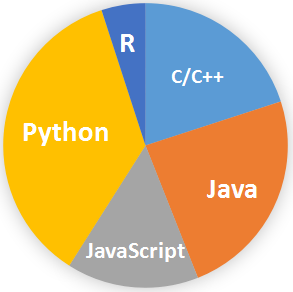
\includegraphics[scale=0.5]{img/languages.png}
    ~
  \section{Tools}
    \textbf{AI Tools} {Numpy, Jupyter Notebook, Conda}
    \textbf{\\Web Technologies} {HTML, CSS, JavaScript, jQuery, Bootstrap, Django}
    \textbf{\\Version Control} {Git}
    \textbf{\\Text Editors} {Visual Studio Code, Brackets}
    \textbf{\\Operating Systems} {Windows, GNU/Linux, Android}
    ~
  \section{Languages}
    \textbf{English}
\includegraphics[scale=0.40]{img/4stars.png}
    \textbf{Hindi}
\includegraphics[scale=0.40]{img/3stars.png}
    ~
\end{aside}

\section{Experience}
\begin{entrylist}
    \entry
    {Feb - Apr, \\ 2018}
    {Summer Intern}
    {AscentSpark, Kolkata, India}
    {Automated Text Writeups Composition: Composing One-Liners From on Public Data on Social-Media Activities of Users.}
\end{entrylist}

\section{Education}
\begin{entrylist}
  \entry
    {2015 - 2019}
    {B. Tech Degree in Computer Science \& Engineering\\}
    {University of Engineering \& Management, Kolkata}
    {Main subjects: \\
        • Artificial Intelligence \qquad \qquad \qquad
        • Data Structures and Algorithms\\
        • Data Science and Analytics \quad \quad \hspace{1mm}
        • Objected Oriented Programming\\
        • Engineering Mathematics
    }
  \entry
    {2014}
    {High School - Class XII}
    {St. Sebastian's School, Kolkata, India}
    {Main subjects: Mathematics, Physics, Computer Science, Chemistry.}
   \entry
    {2012}
    {Secondary School - Class X}
    {St. Sebastian's School, Kolkata, India}
    {Main subjects: Mathematics, Physics, Computer Applications, Chemistry.}
\end{entrylist}

\section{Projects}
\begin{entrylist}
  \entry
    {07/2017}
    {Sudoku Solver}
    {Udacity}
    {\emph{AI agent written in Python / Pygame to solve Sudoku puzzles.}}
  \entry
    {10/2017}
    {Banking System}
    {UEM, Kolkata}
    {\emph{Online Banking System web-app written in Django.}}
  \entry
    {03/2018}
    {Unix Shell Emulator}
    {UEM, Kolkata}
    {\emph{Emulates a simple UNIX shell in a Linux environment.}}
    
\end{entrylist}

\section{Areas of Interest}
\begin{itemize}
    \item Artificial Intelligence, Machine Learning, Deep Learning
    \item Deep Reinforcement Learning
    \item Data Visualization
    \item Web Development
\end{itemize}

\section{Certifications}
\begin{entrylist}
  \entry
    {02/2018}
    {Neural Networks and Deep Learning}
    {deeplearning.ai, Coursera}
    {\emph{Building an Image Classifier}}
  \entry
    {06/2018}
    {Data Science: Visualization}
    {Harvard University, edX}
    {\emph{Using ggplot2 in R to visualize datasets and draw inferences}}
  \entry
    {03/2017}
    {Programming, Data Structures and Algorithms in Python\\}
    {IIT-Madras, NPTEL}
    
\end{entrylist}
\end{document}